\chapter[Desenvolvimento]{Desenvolvimento}

\section{Cenário Modelo}

\subsection{Caso 1}

Agentes envolvidos: Carro C1 e Carro C3, ambos representam as categorias de
automóveis que se enquadram no uso do CIAC e Carro C2, representa um carro
modelo Gol G3/G4 1.0.

Situação: Carro C2 deseja ultrapassar o Carro C1 e o Carro C3 trafega na mesma
via em sentido oposto como mostra a imagem \ref{fig:caso1} a seguir.

\begin{figure}[h]
  \centering
  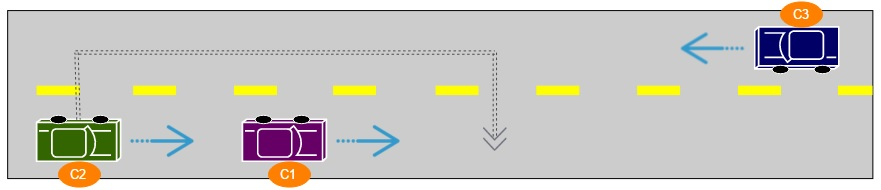
\includegraphics[width=400px, scale=1]{figuras/caso1}
  \caption{Demonstração do Caso 1}
\label{fig:caso1}
\end{figure}

Procedimentos:

\begin{enumerate}
  \item O CIAC identificará a intenção de ultrapassagem do condutor do Carro
  C2 que acionará o sistema por completo, monitorando as seguintes situações:
  \begin{itemize}
    \item Acionamento da seta;
    \item Mudança na angulação do volante, utilizando o sensor de rotação PST-360;
    \item Mudança de faixa, utilizando a câmera AWS650;
    \item Quando a distância entre o Carro C2 e o Carro C1 diminuir, utilizando a
    câmera AWS650, o Lidar HDL-64E e o Radar ARS-30X.
  \end{itemize}

  \item Em seguida, o sistema irá verificar se há presença de algum automóvel
  trafegando na mesma via em sentido oposto, fazendo uso da câmera AWS650, do
  Lidar HDL-64E e do Radar ARS-30X;

  \item Havendo a presença de um automóvel, nesse caso o Carro C3, o CIAC identificará:
  \begin{itemize}
    \item Posição geográfica do Carro C3, por meio da utilização do GPS
    A2100-A/B, do Radar ARS-30X e do Lidar HDL-64E;

    \item Velocidade do Carro C3, empregando o par Tranponder-Velocímetro do
    veículo, o Radar ARS-30X e o Lidar HDL-64E.
    \begin{itemize}
      \item Quando o CIAC identificar a intenção do condutor de realizar uma
      ultrapassagem, o transponder emitirá um sinal “questionador” do Carro C2
      para o Carro C3, solicitando, através da emissão de radiofrequência, a
      posição geográfica e a velocidade do Carro C3, dados que serão fornecidos
      pelo GPS e velocímetro do carro, respectivamente;

      \item E simultaneamente, a velocidade do Carro C3, a distância entre os
      carros C2 e C3 e tempo de encontro entre os mesmos estarão sendo aferidos
      com o auxílio do Radar, o qual emite ondas de rádio do Carro C2 que serão
      refletidas pelo Carro C3 e baseado no tempo de ida e volta do sinal
      obtêm-se a distância entre os dois carros, a velocidade do Carro C3 e
      assim, o tempo de encontro do Carro C2 com o Carro C3;

      \item E o Lidar, dispositivos que funciona com a emissão de um laser do
      Carro C2 que será refletido pelo Carro C3 e através do tempo de ida e
      volta desses pulsos é calculada a distância entre os carros C2 e C3.

    \end{itemize}
  \end{itemize}
\end{enumerate}
